\chapter{Firmware inerciální jednotky}
Firmware hlavního \ac{MCU} byl vyvíjen pomocí volně dostupného \ac{IDE} poskytovaného výrobcem - \emph{STM32CubeIDE}. Jedná se o nástroj určený pro práci s jazyky C/C++, GCC kompilátorem založeném na Eclipse \cite{V2Tf5wsrbWcbQdoW}. Zároveň poskytuje grafické rozhraní pro konfiguraci a generování knihoven založených na \ac{HAL}, možnost použití \ac{RTOS} a ladící prostředí.

V této práci byly použity poskytované knihovny HAL a FreeRTOS pro ulehčení a urychlení vývoje firmwaru. Jejich použití často s sebou nese nevýhody, jako je například horší využití paměti, nebo výpočetního výkonu, z tohoto důvodu byl zvolen takový \ac{MCU}, aby měl dostatečné rezervy pro jejich použití.
\section{HAL}
Generování kódu \ac{HAL} v  STM32CubeIDE je možné pomocí grafického rozhraní, které poskytuje uživateli možnost nastavení jednotlivých pinů, periferií, komunikačních rozhraní a vnitřních hodin (obrázek \ref{fig:cubeConfig}). Vygenerované knihovny následně umožňují uživateli pracovat s \ac{MCU} s jistou mírou abstrakce, například není nutné znát a pracovat s názvy jednotlivých registrů. Typickým příkladem můžou být komunikační sběrnice (\ac{SPI}, \ac{I2C} \ldots), pro které jsou dostupné obslužné funkce na čtení a vysílání dat, jak v blokujícím režimu, tak i v neblokujícím (například pomocí \ac{DMA}). \cite{V2Tf5wsrbWcbQdoW}

Dále je možné pomocí stejného grafického rozhraní importovat rozšiřující softwarové balíčky, i když už se nejedná přímo o \ac{HAL}. V této práci byly použity \emph{FATFS} pro manipulaci se soubory na microSD kartě, \emph{FreeRTOS} jakožto jeden z dostupných \ac{RTOS} a \emph{USB\_DEVICE} pro práci s \ac{USB} rozhraním třídy \ac{MSC}.

\begin{figure}[h]
     \centering
     \begin{subfigure}[b]{0.4\textwidth}
         \centering
         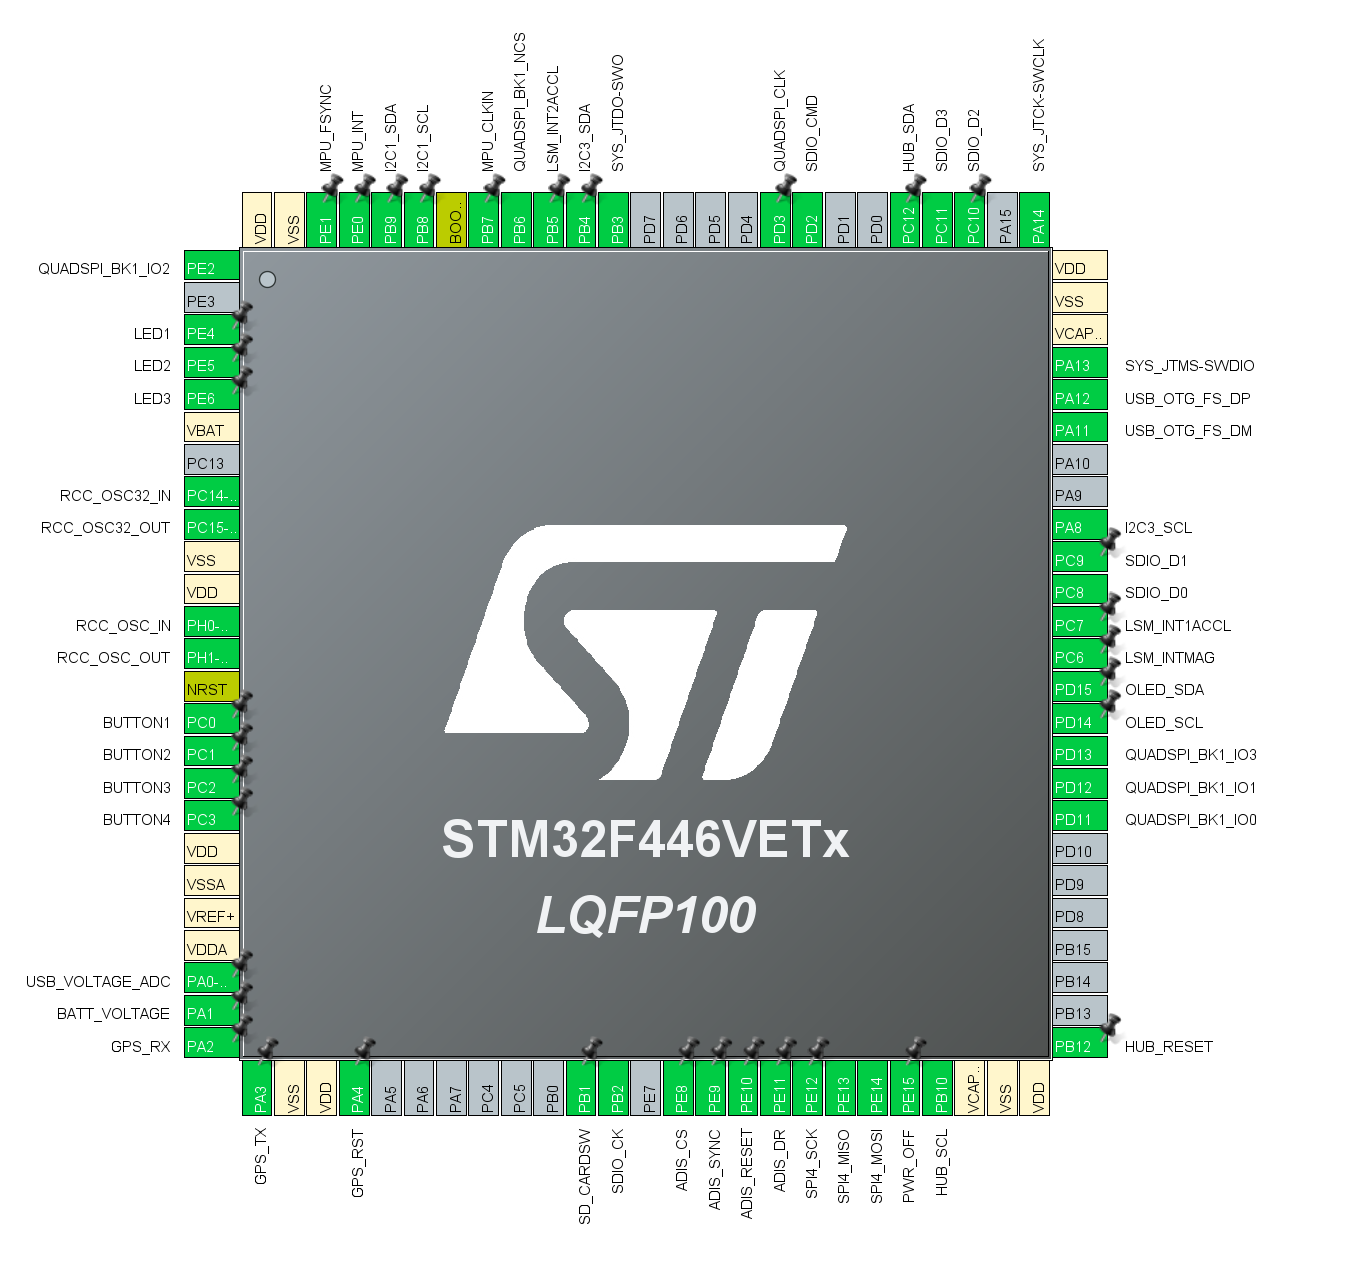
\includegraphics[width=\textwidth]{obrazky/cubePinout}
         \caption{Konfigurace pinů}
       
     \end{subfigure}
     \hfill
     \begin{subfigure}[b]{0.4\textwidth}
         \centering
         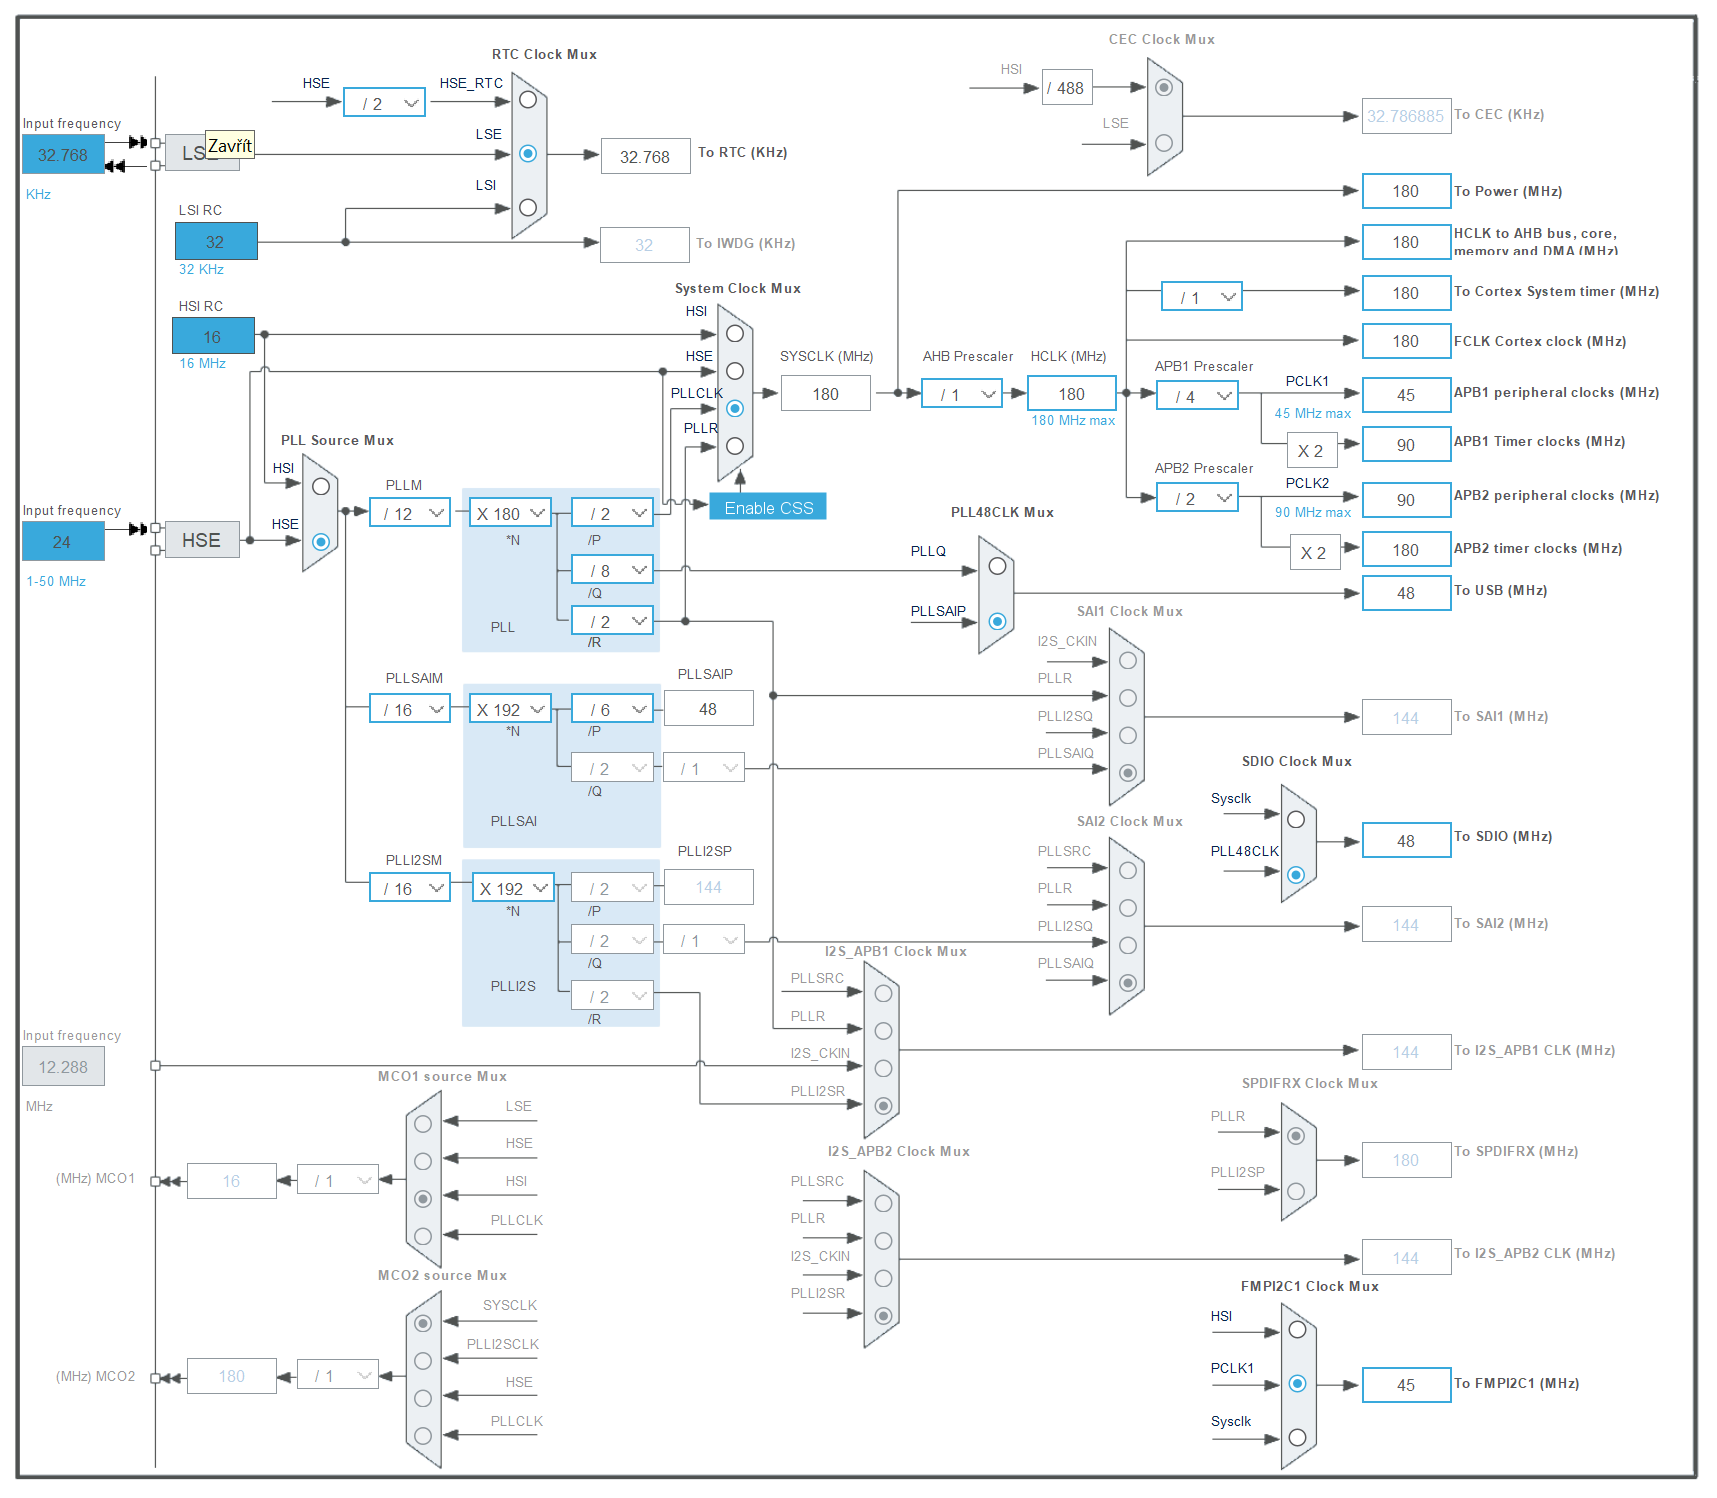
\includegraphics[width=\textwidth]{obrazky/cubeClock}
         \caption{Konfigurace hodin}
         
     \end{subfigure}
        \caption{Konfigurace MCU v STM32CubeIDE}
        \label{fig:cubeConfig}
\end{figure}

\section{FreeRTOS}
V této aplikaci je potřeba vyčítat, převádět a zapisovat data z několika různých senzorů které nemají přesně stejný hodinový signál, zároveň obsluhovat \ac{GUI} a provádět záznam dat zároveň. Pro potřeby synchronizace několika úloh, které nemají stejné periody, nebo například čekají na vstup od uživatele se hodí \ac{RTOS}.

Byla vybrána jedna z variant operačních systémů reálného času, a to FreeRTOS. Jedná se o jednoduchý open-source systém, který je hojně využíván ve vestavěných aplikacích. Umožňuje aplikaci virtuálně rozdělit na několik samostatných vláken (tzv. \emph{tasků}) s různými prioritami. Časování tasků je možné například pomocí neblokujících prodlev, nebo semaforů. FreeRTOS také plní funkci správy a alokace paměti. Předávání informací mezi jednotlivými tasky se provádí pomocí tzv. \emph{Queues}, které představují \ac{FIFO} zásobníky s nastavitelnou délkou fronty a velikosti jednotlivých dat. Díky tomu je možné se vyvarovat použití globálních proměnných. \cite{Zhu2011}

Práce s FreeRTOS je v STM32CubeIDE zjednodušená také díky poměrně dobré možnosti ladit aplikace pomocí již vestavěného RTOS-aware debuggeru, díky kterému můžeme například analyzovat využití paměti jednotlivých tasků, využití času, nebo kontrolovat stavy semaforů a velikost obsazených Queues. 

\section{Vývojové diagramy firmwaru}
Popsat chování a funkcionalitu firmwaru této aplikace dohromady by bylo poměrně nepřehledné. Proto budou jednotlivé funkce rozděleny do několika samostatných logických bloků, kde každý blok reprezentuje jeden task operačního systému.

\subsection{KeepaliveTask}
\begin{figure}[h]
    \centering
    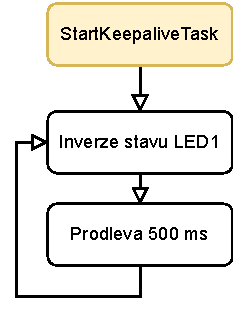
\includegraphics[width=0.25\textwidth]{obrazky/KeepaliveTask}
    \caption{Vývojový diagram KeepaliveTask}
\end{figure}
Jedná se o úlohu s nastavenou nejnižší prioritou. Slouží pouze pro ladicí účely a umožňuje jednoduchou a rychlou reprezentaci stavu systému pomocí blikající LED, zdali je spouštěn i task s nejnižší prioritou.
\subsection{hubTask}
\begin{figure}[h]
    \centering
    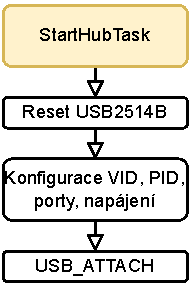
\includegraphics[width=0.2\textwidth]{obrazky/HubTask}
    \caption{Vývojový diagram HubTask}
\end{figure}
Tato úloha vykonává funkce pouze při zapnutí zařízení, a to konfiguraci a sepnutí vestavěného \ac{USB} rozbočovače. Do něj jsou nahrána konfigurační data pomocí sběrnice I2C, jako je například \ac{VID}, \ac{PID} a nastavení jednotlivých portů. Následně jsou registry rozbočovače přepnuty do režimu pouze pro čtení a \ac{USB} rozhraní zapnuto.
\subsection{powerTask}
V tomto tasku jsou periodicky měřena všechna analogová napětí pomocí \ac{ADC} procesoru, například napětí zdroje, USB portu, akumulátoru, ale i teplota procesoru. Tyto stavové veličiny jsou zobrazovány pomocí \ac{GUI}. Čtené hodnoty napětí akumulátoru jsou průměrovány pomocí pohyblivého exponenciálního filtru, který je možný zapsat pomocí rovnice \ref{eq:EMA}.

\begin{equation} \label{eq:EMA}
y[n]=\alpha \cdot x[n] + (1-\alpha)\cdot y[n-1]
\end{equation}

Kde $ x[n] $ je přečtená hodnota napětí, $ y[n] $ vyfiltrovaná hodnota napětí, $ y[n-1] $ výsledek vyfiltrované hodnoty napětí z předešlého cyklu a $ \alpha $ je nastavitelný koeficient odezvy filtru. Experimentálně bylo odzkoušeno, že vhodných výsledků filtrace šumu je možné dosáhnout s $ \alpha = 0,3$. Tento typ filtru byl zvolen zejména pro jeho jednoduchost a úsporné využití paměti.

V případě, že klesne napětí akumulátoru pod hranici 3,5 V je zařízení vypnuto překlopením S/R klopného obvodu, který je zmiňovaný v kapitole \ref{hardware} a tím je dosažena ochrana akumulátoru proti podvybití.


\begin{figure}[h]
    \centering
    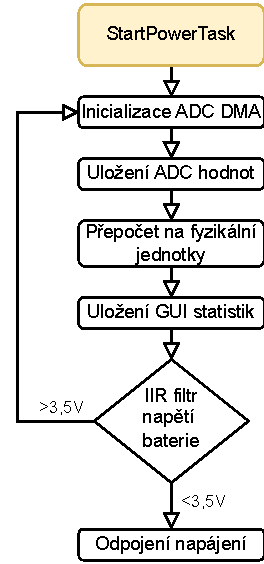
\includegraphics[width=0.3\textwidth]{obrazky/PowerTask}
    \caption{Vývojový diagram PowerTask}
\end{figure}
\subsection{gpsTask}
Tato úloha se stará o periodické zpracování příchozích dat z GNSS modulu pomocí \ac{UBX} zpráv. Tyto data jsou přijímány pomocí sběrnice \ac{UART} a DMA, následně převedena do čitelné podoby (datum, čas, zeměpisná šířka, délka \ldots) pomocí knihovny GNSS parseru z \cite{SimpleMethod2021}.

V této úloze je také kontrolováno kdy dojde k prvnímu přesnému určení polohy fixací na satelity a je aktualizován aktuální čas a datum do vnitřního \ac{RTC}.
\begin{figure}[h]
    \centering
    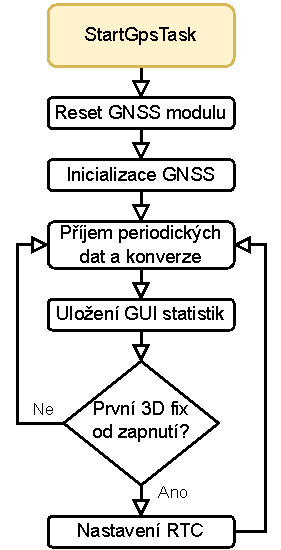
\includegraphics[width=0.3\textwidth]{obrazky/GpsTask}
    \caption{Vývojový diagram GpsTask}
\end{figure}
\subsection{lsmTask} \label{lsmTask}
V tomto tasku jsou periodicky vyčítána data o magnetickém poli z elektronického kompasu LSM303. Ten je při zapnutí zresetován a následně inicializován rozsah, rozlišení a vzorkovací frekvence na 100 Hz. Po navzorkování dat magnetometr změní stav na svém pinu signalizujícím konec vzorkování. V ten okamžik je započat DMA přenos pomocí sběrnice I2C a jakmile jsou data vyčtena, převedou se do fyzikálních jednotek a odešlou se k záznamu.
\begin{figure}[h]
    \centering
    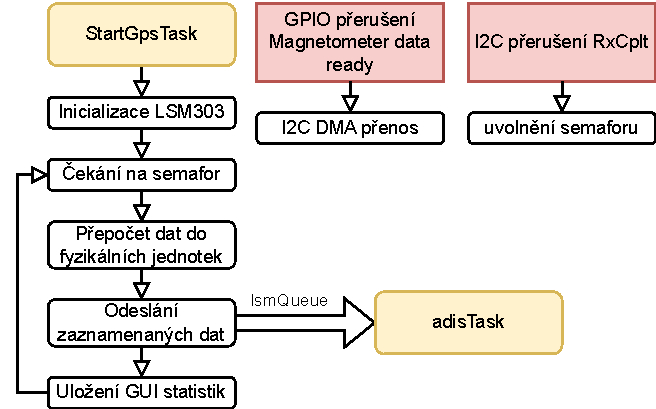
\includegraphics[width=0.6\textwidth]{obrazky/LsmTask}
    \caption{Vývojový diagram LsmTask}
\end{figure}
\subsection{mpuTask}
Tato úloha je velice obdobná předchozí z kapitoly \ref{lsmTask}. Zde jsou čtena a převáděna data z 6 osého IMU MPU6050 s frekvencí 400 Hz.
\begin{figure}[h]
    \centering
    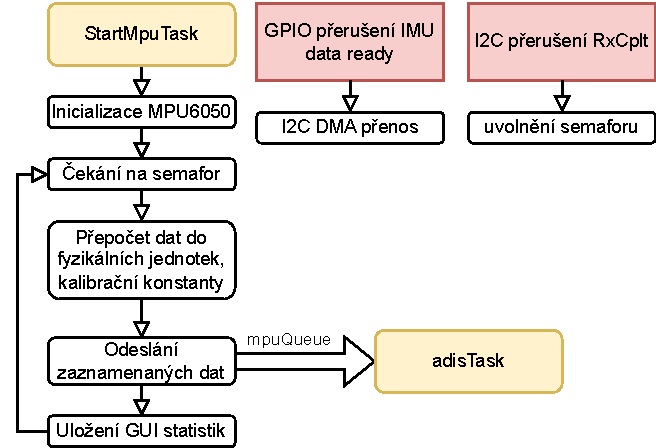
\includegraphics[width=0.6\textwidth]{obrazky/MpuTask}
    \caption{Vývojový diagram MpuTask}
\end{figure}
\subsection{adisTask}
Tento task, obdobně jako předchozí, obstarává inicializaci, vyčítání a konverzi dat z 6 osého IMU ADIS16505 se vzorkovací frekvencí 400 Hz. Zároveň slouží jako synchronizace k zarovnání řádků dat ve výsledném souboru. V případě, že jsou dostupná nová data z LSM303, nebo MPU6050, jsou přidána do celkové záznamové datové struktury, v opačném případě jsou na jejich odpovídající místa zapsány nuly. V nejhorším možném případě, tedy že data z ostatních senzorů jsou vzorkována těsně po navzorkování dat z ADIS16505 je jejich zpoždění délka jedné periody celkové vzorkovací frekvence, tedy 2,5 ms.
\begin{figure}[h]
    \centering
    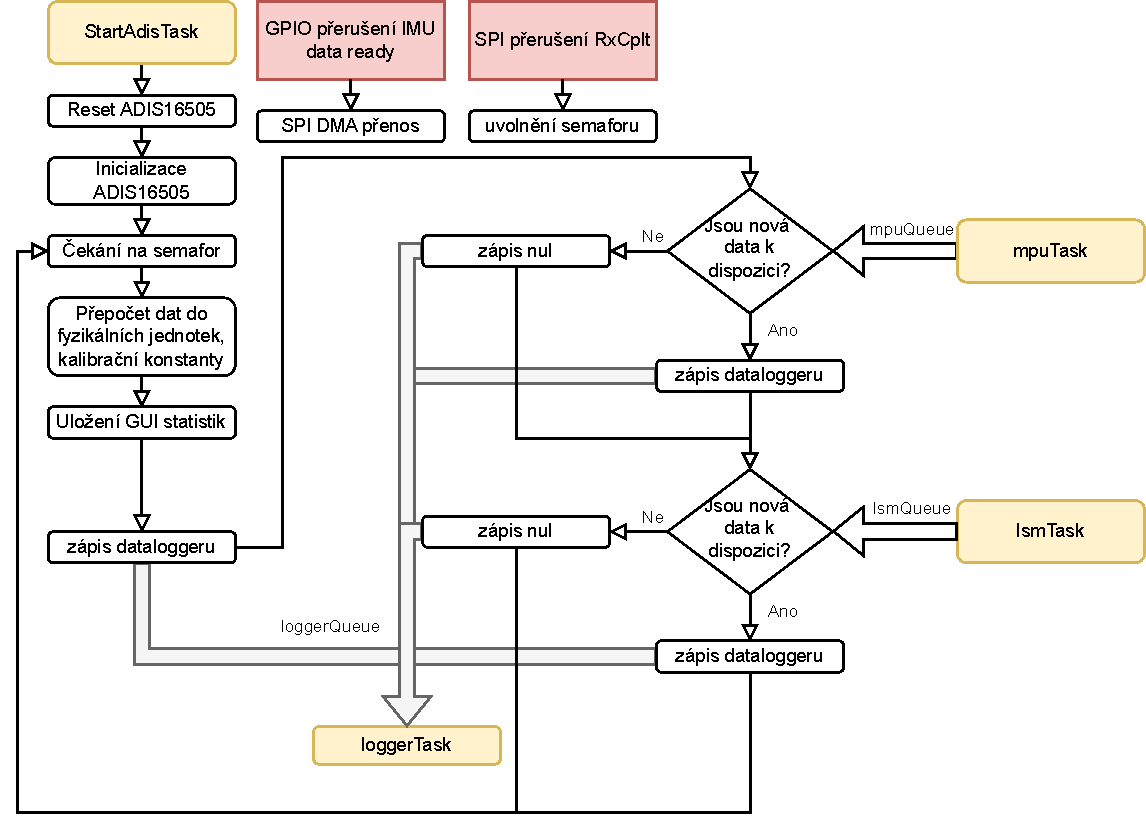
\includegraphics[width=0.95\textwidth]{obrazky/AdisTask}
    \caption{Vývojový diagram AdisTask}
\end{figure}
\subsection{loggerTask}
Tato úloha provádí samotné ukládání dat. Testováním bylo zjištěno, že při použití kvalitnějších microSD karet (v zařízení je použita \emph{SAMSUNG 64GB EVO PLUS}) nedochází k náhodným delším prodlevám při zápisu. Zároveň v porovnání s NOR FLASH pamětí poskytuje řádově větší úložiště, rychlejší zápis bloku dat, není potřeba mazat každý sektor paměti před zápisem a také je jednoduší implementace souborového systému. Z těchto důvodů bylo rozhodnuto využití SD karty k ukládání měřených dat.

Stavový automat v tomto tasku lze rozdělit do čtyř stavů: záznam dat, kdy jsou data průběžně ukládána, vypnutý záznam, kdy jsou data zahazována a začátek a konec záznamu, kdy dochází k inicializacím USB a souborových systémů. V průběhu záznamu je USB rozhraní vypnuté, aby nebylo možné zasahovat do souboru připojeným PC když je zrovna do něj zapisováno zařízením.

Samotný přenos naměřených dat do počítače je realizován přes USB třídy vysokokapacitního úložiště. Připojený PC při potřebě čtení dat spustí přerušení na přenos s konkrétní adresou. Jelikož je na microSD kartě implementován souborový systém FatFS, je v běžných operačních systémech reprezentován jako obyčejné externí úložiště.
\begin{figure}[h]
    \centering
    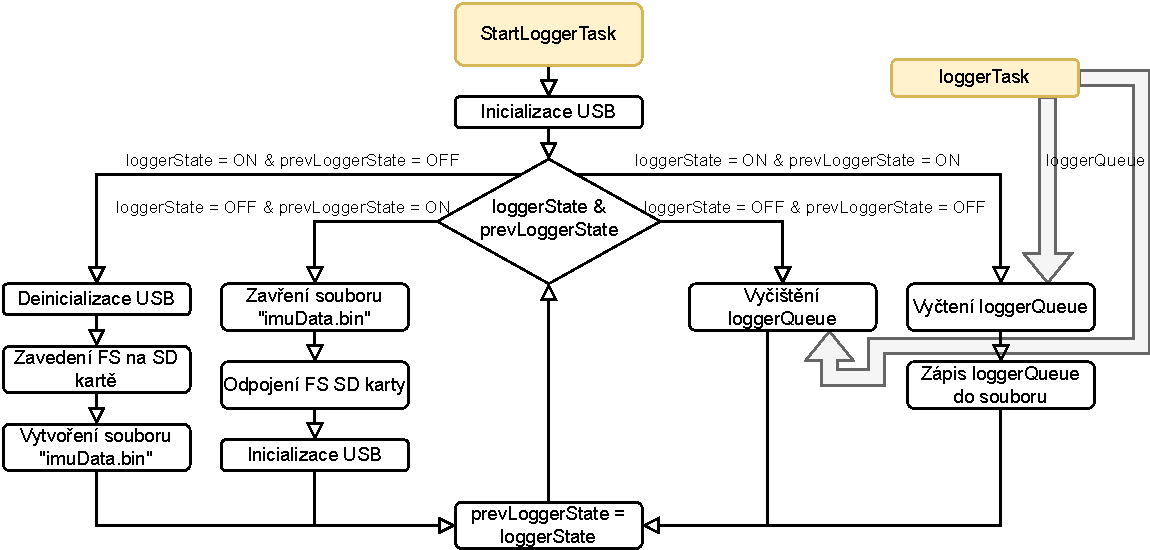
\includegraphics[width=0.99\textwidth]{obrazky/LoggerTask}
    \caption{Vývojový diagram LoggerTask}
\end{figure}
\subsection{oledTask}
\begin{figure}[h]
    \centering
    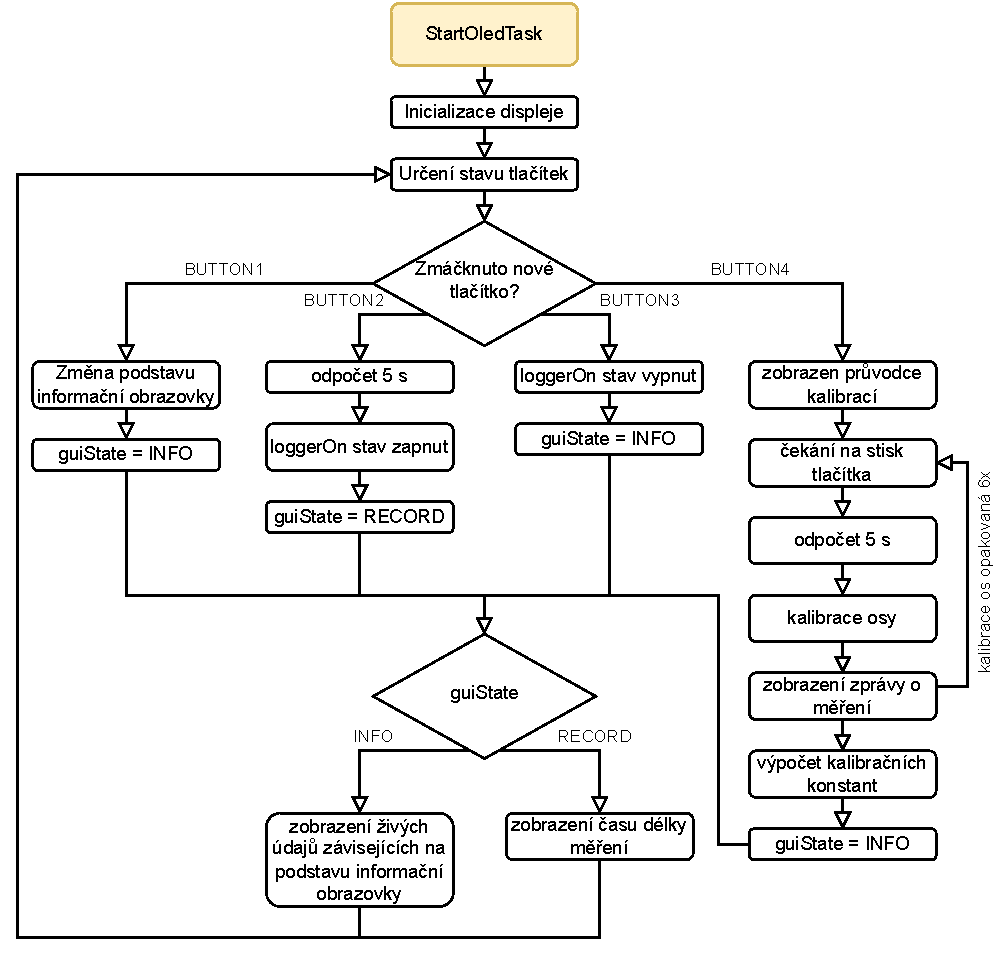
\includegraphics[width=0.9\textwidth]{obrazky/OledTask}
    \caption{Vývojový diagram OledTask}
\end{figure}

\section{Kalibrace IMU}
\section{Zarovnání paměti}



